\documentclass{ximera}

\usepackage{microtype}
\usepackage{tikz}
\usepackage{tkz-euclide}
\usetkzobj{all}
\tikzstyle geometryDiagrams=[ultra thick,color=blue!50!black]

\renewcommand{\epsilon}{\varepsilon}



\title{Stereographic projection}
\begin{document}
\begin{abstract}
Here we start to develop another model for our geometry.
\end{abstract}
\maketitle


\subsection*{Stereographic projection coordinates}

Now let's project $K$-geometry,
\[
1=K\left(x^{2}+y^{2}\right)+z^{2} 
\]
onto the plane $z=1$ using the `South Pole' $S=(0,0,-1)$ as the center of
projection:
\begin{image}
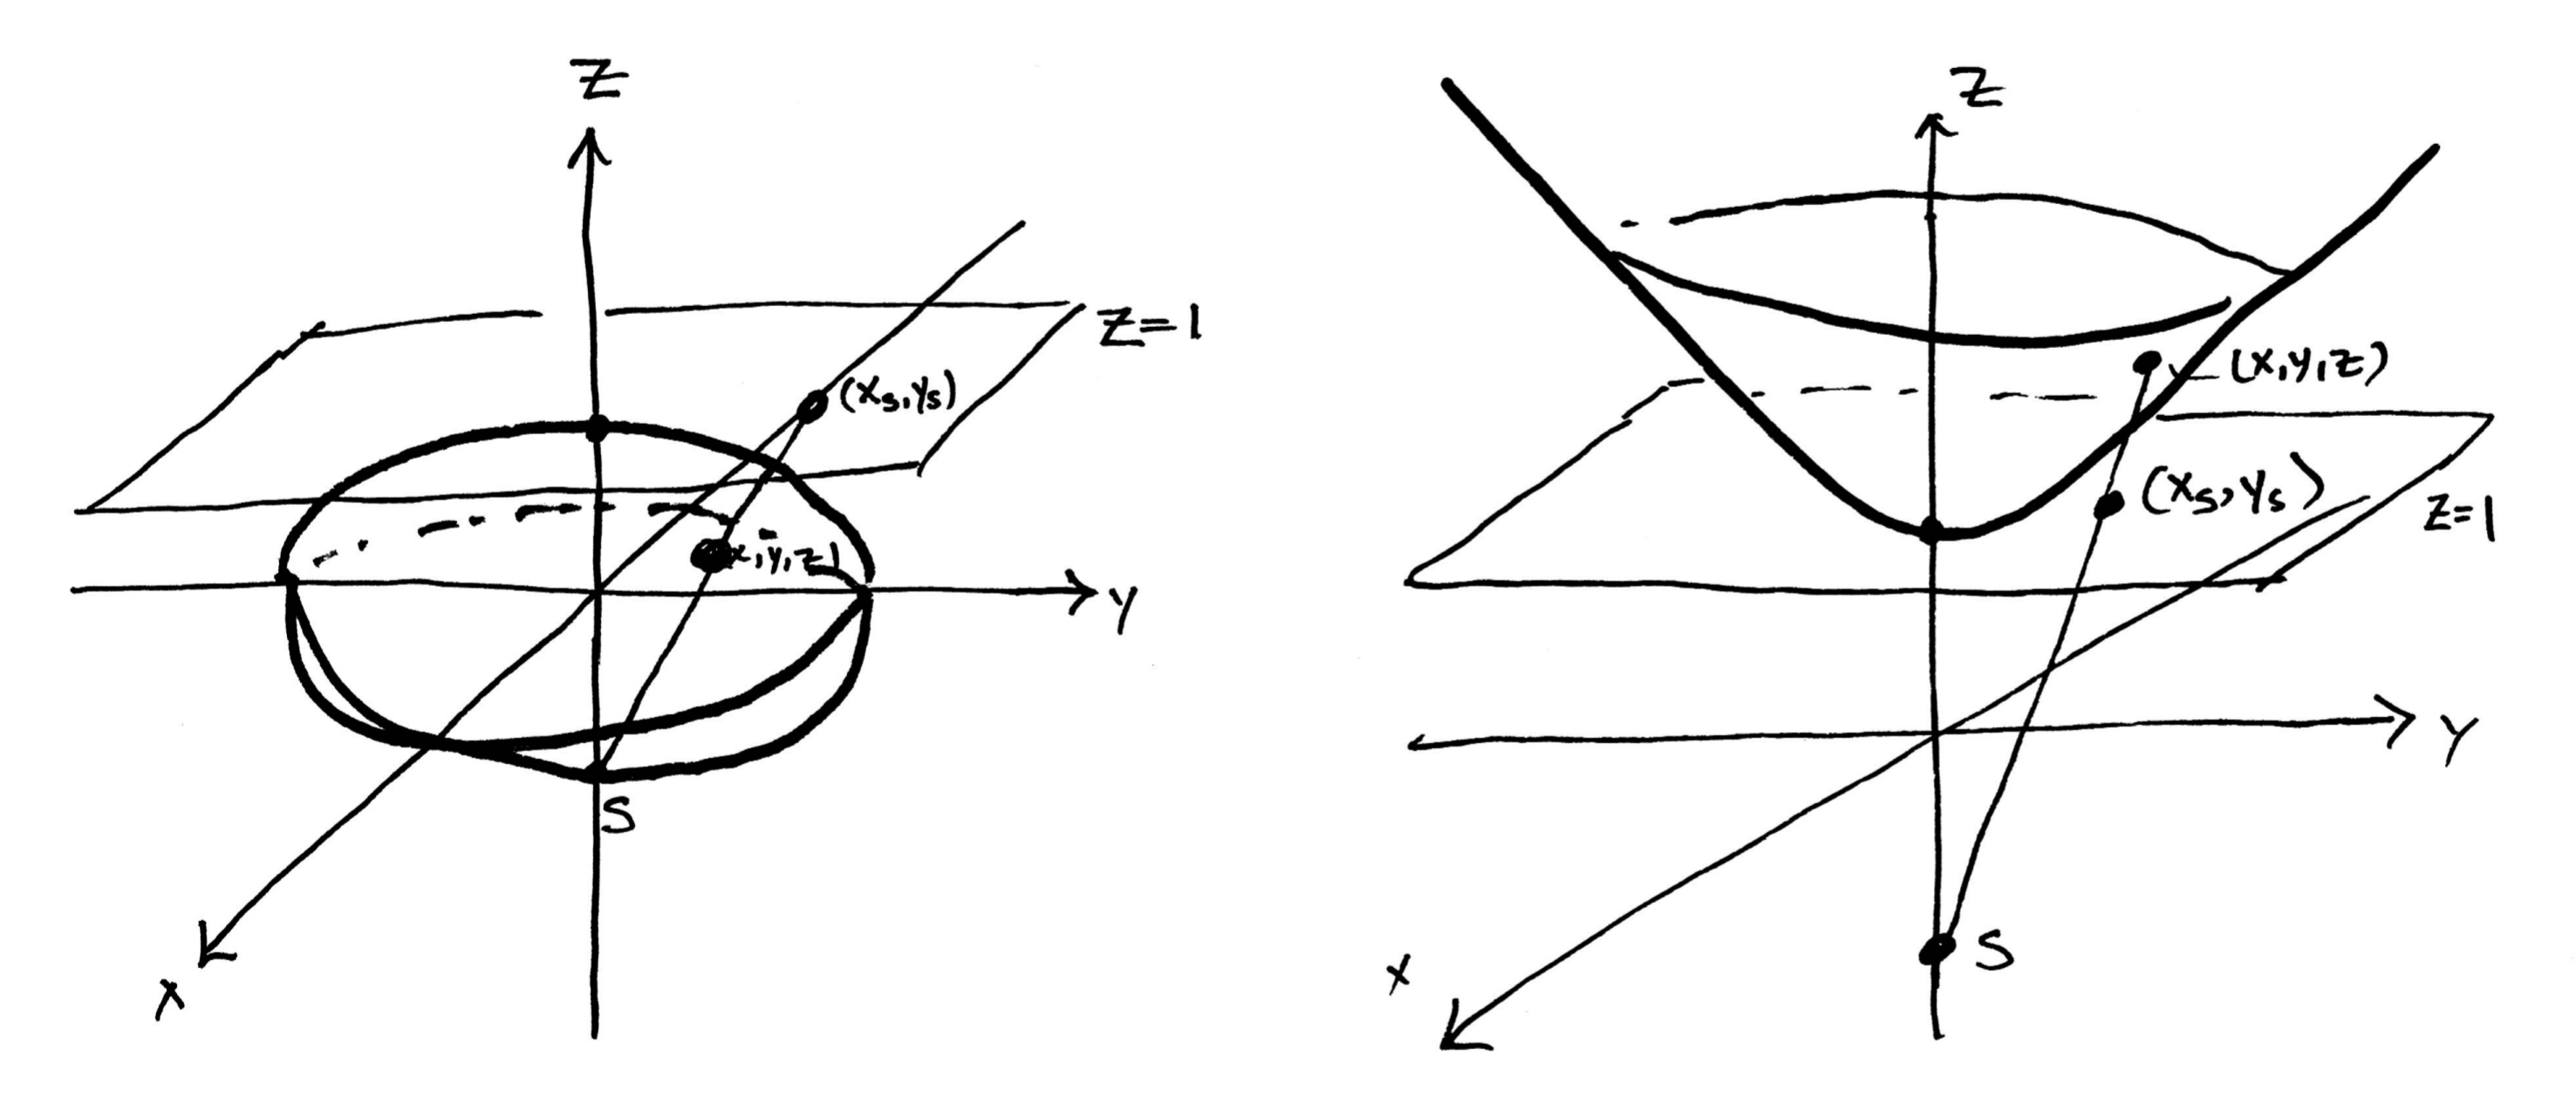
\includegraphics[width=5in]{stereoProj.png}
\end{image}
Let's look at this from a different vantage point, say with our eye
along the edge of the plane $z=1$:
\begin{image}
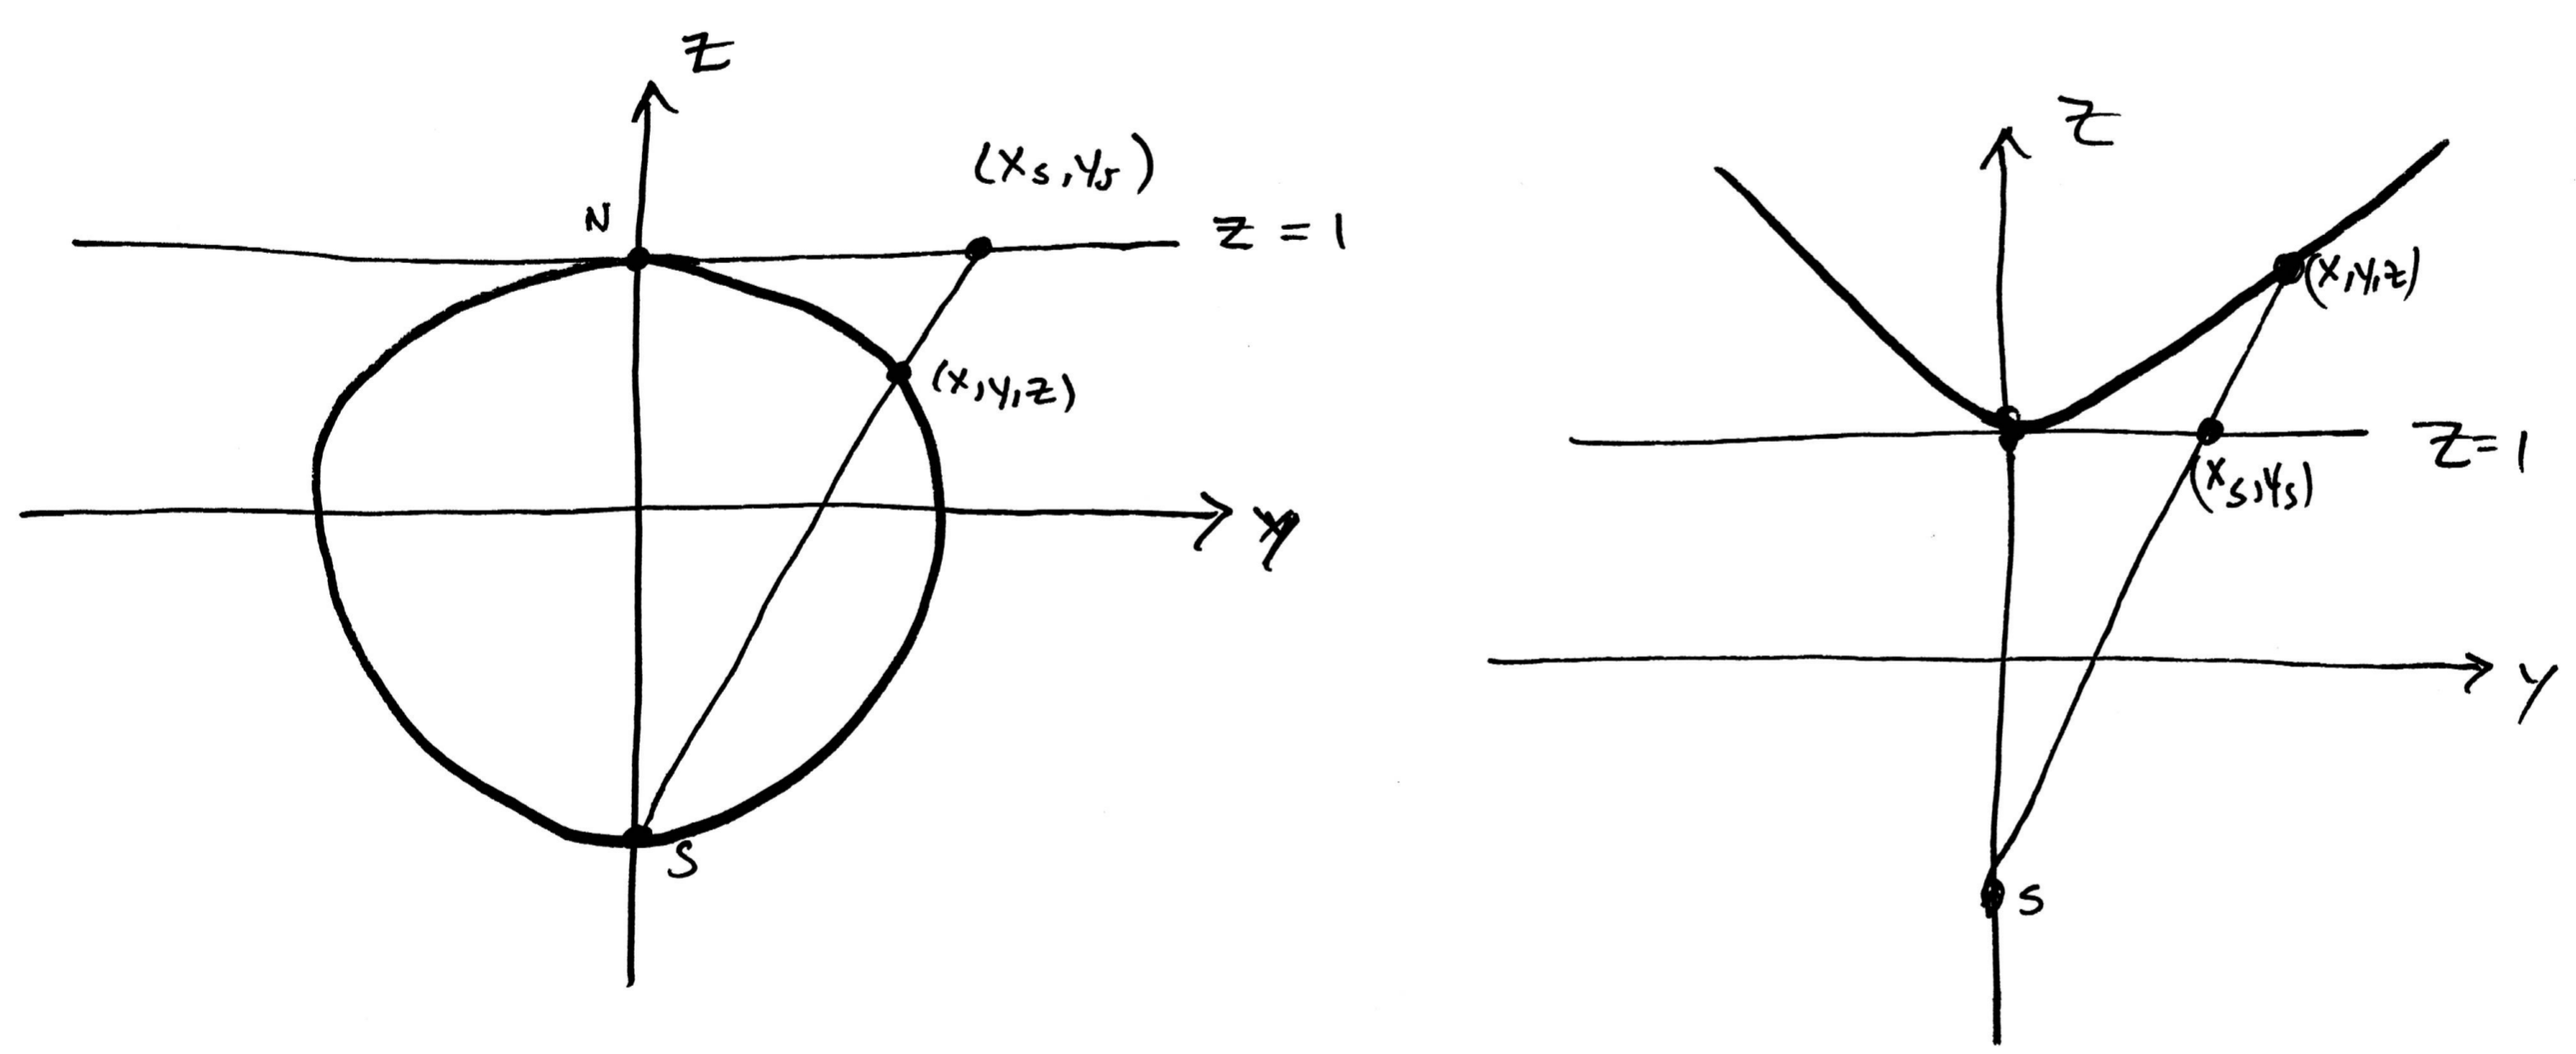
\includegraphics[width=5in]{stereoCross.png}
\end{image}

\begin{problem}
  If $K=1$ where does the `equator' map to? What about the `Northern hemisphere?' How about the `Southern hemisphere?'
  \begin{freeResponse}
    The `equator' maps to the circle of radius $2$ centered at the
    origin in the $(x_s,y_s)$ plane.  The `Northern hemisphere' maps
    inside this circle, and the `Southern hemisphere' maps outside the
    circle.
  \end{freeResponse}
\end{problem}

\begin{problem}
  Use similar triangles to explain why there is a number $\rho$ such
  that for any given $(x,y,z)$
  \[
  \rho\cdot(x_s,y_s,2) = (x,y,z+1).
  \]
  \begin{freeResponse}
    Let $A = (x,y,z)$, $B= (x,y,-1)$, $A_s = (x_s,y_s,1)$ and
    $B_s=(x_s,y_s,-1)$. From the diagram above we see that
    \[
    \angle ASB = \angle A_s S B_s.
    \]
    Moreover, since $\triangle ASB$ and $\triangle A_s S B_s$ are
    right triangles, we now see that two of their angles have the same
    measure, and hence all three have the same measure. This means
    that these triangles are similar, and hence there they are
    dilations of one another. Hence there is a scale-factor $\rho$
    such that
    \[
    \rho\cdot(x_s,y_s,2) = (x,y,z+1).
    \]
  \end{freeResponse}
\end{problem}

\begin{problem}
  For the projection of the set $1=K\left(x^{2}+y^{2}\right)+z^{2}$
  onto the $z=1$ plane with center of projection $S$, write
  $(x_{s},y_{s})$ as a function of $(x,y,z)$.
  \begin{freeResponse}
    We know that
    \[
    \rho\cdot(x_{s},y_{s},2)=(x,y,z+1),
    \]
    hence $\rho=\frac{z+1}{2}$, and we may now write
    \begin{align*}
      x_{s} &=\frac{2x}{z+1},\\
      y_{s} &=\frac{2y}{z+1}.
    \end{align*}
  \end{freeResponse}
\end{problem}

\begin{problem}
  For the projection of the set $1=K\left(x^{2}+y^{2}\right)+z^{2}$
  onto the $z=1$ plane with center of projection $S$, write
  $(x,y,z)$ as a function of $(x_s,y_s)$.
  \begin{hint}
    Note that
      \[
      \rho\cdot(x_{s},y_{s},2)=(x,y,z+1) \qquad\text{and}\qquad z = 2\rho-1.
      \]
  \end{hint}
  \begin{hint}
    Hence if
    \[
    1 = K\left(x^2 + y^2\right) + z^2
    \]
    we may write
    \[
    1 = K\left((\rho\cdot x_s)^2 + (\rho\cdot y_s)^2\right) + (2\rho-1)^2
    \]
    and solve for $\rho$.
  \end{hint}
  \begin{freeResponse}
    This is slightly more complex than the previous problem; however,
    we will begin the same way. We know that
    \[
    \rho\cdot(x_{s},y_{s},2)=(x,y,z+1),
    \]
    hence $\rho=\frac{z+1}{2}$, and we may now write
    \begin{align*}
      x &= \rho \cdot x_s,\\
      y &= \rho \cdot y_s,\\
      z &= 2\rho-1.
    \end{align*}
    Now our task is now to write $\rho$ in terms of $x_s$ and
    $y_s$. Using our assignments above, write
    \begin{align*}
      1 &= K\left(x^2 + y^2\right) + z^2\\
      1 &= K\left((\rho\cdot x_s)^2 + (\rho\cdot y_s)^2\right) + (2\rho-1)^2\\
      1 &= K\left((\rho\cdot x_s)^2 + (\rho\cdot y_s)^2\right) + 4\rho^2-4\rho + 1\\
    \end{align*}
    and so
    \begin{align*}
      0 &= K\left((\rho\cdot x_s)^2 + (\rho\cdot y_s)^2\right) + 4\rho^2-4\rho\\
      0 &= \rho^2\cdot K\left(x_s^2 + y_s^2\right) + 4\rho^2-4\rho
    \end{align*}
    and since $\rho \ne 0$, we may write
    \begin{align*}
      \rho\cdot K\left(x_s^2 + y_s^2\right) + 4\rho-4 &=0 \\
      \rho\left(K\left(x_s^2 + y_s^2\right) + 4\right) &=4\\
      \rho &= \frac{4}{K\left(x_s^2 + y_s^2\right) + 4}.
    \end{align*}
    Hence
    \begin{align*}
      x &= \frac{4x_s}{K\left(x_s^2 + y_s^2\right) + 4},\\
      y &= \frac{4y_s}{K\left(x_s^2 + y_s^2\right) + 4},\\
      z &= \frac{4-K\left(x_s^2 + y_s^2\right)}{4+K\left(x_s^2 + y_s^2\right)}.\\
    \end{align*}
  \end{freeResponse}
\end{problem}


\section{Stereographic projection dot product}

Once more, we want to be able to find a dot product that will allow us
to compute lengths in stereographic projection coordinates that will agree
with the $K$-dot product, and hence the euclidean dot product.

\begin{problem}
Suppose we have a curve $X$ in $K$-warped space that is a function of
a curve $X_s$ in the plane $z=1$ space. So
\[
X_s(t) = \left( x_s(t),y_s(t)\right)
\]
and
\[
X(t) = 
\begin{cases}
  x(x_s(t),y_s(t)),\\
  y(x_s(t),y_s(t)),\\
  z(x_s(t),y_s(t)).
\end{cases}
\]
Use the chain rule to compute
\[
\dd[x]{t}, \qquad \dd[y]{t}, \qquad \dd[z]{t},
\]
in terms of $\dd[x_s]{t}$, $\dd[y_s]{t}$, $\pp[x]{x_s}$,
$\pp[y]{x_s}$, $\pp[z]{x_s}$, $\pp[x]{y_s}$, $\pp[y]{y_s}$,
and $\pp[z]{y_s}$.
  \begin{hint}
  Simply write down the answer from a previous problem with some minor
  changes.
  \end{hint}
  \begin{freeResponse}
  Write
  \begin{align*}
    \dd[x]{t} &= \begin{bmatrix}\pp[x]{x_s} & \pp[x]{y_s}\end{bmatrix}\cdot\begin{bmatrix}\dd[x_s]{t} & \dd[y_s]{t}\end{bmatrix}^\transpose = \pp[x]{x_s}\cdot\dd[x_s]{t}+\pp[x]{y_s}\cdot\dd[y_s]{t} &  \\
    \dd[y]{t} &= \begin{bmatrix}\pp[y]{x_s} & \pp[y]{y_s}\end{bmatrix}\cdot\begin{bmatrix}\dd[x_s]{t} & \dd[y_s]{t}\end{bmatrix}^\transpose = \pp[y]{x_s}\cdot\dd[x_s]{t}+\pp[y]{y_s}\cdot\dd[y_s]{t} &  \\
    \dd[z]{t} &= \begin{bmatrix}\pp[z]{x_s} & \pp[z]{y_s}\end{bmatrix}\cdot\begin{bmatrix}\dd[x_s]{t} & \dd[y_s]{t}\end{bmatrix}^\transpose = \pp[z]{x_s}\cdot\dd[x_s]{t}+\pp[z]{y_s}\cdot\dd[y_s]{t}.  
  \end{align*}
\end{freeResponse}
\end{problem}


\begin{problem}
  With the same setting as in the previous problem, rewrite the result
  of your computation in matrix notation to find $D_s$
  such that
\[
\begin{bmatrix}
\dd[x]{t} & \dd[y]{t} & \dd[z]{t}
\end{bmatrix}
=
\begin{bmatrix}
\frac{dx_s}{dt} & \frac{dy_s}{dt}
\end{bmatrix}\cdot D_s.
\]
\begin{hint}
  Simply write down the answer from a previous problem with some minor
  changes.
\end{hint}
\begin{freeResponse}
  \[
  D_s =
  \begin{bmatrix}
    \pp[x]{x_s} & \pp[y]{x_s} & \pp[z]{x_s} \\
    \pp[x]{y_s}   & \pp[y]{y_s}   & \pp[z]{y_s}
  \end{bmatrix}.
  \]
\end{freeResponse}
\end{problem}

\begin{problem}
  Now find $P_s$ in terms of $K$, $\pp[x]{x_s}$, $\pp[y]{x_s}$,
  $\pp[z]{x_s}$, $\pp[x]{y_s}$, $\pp[y]{y_s}$, and $\pp[z]{y_s}$ such
  that
  \[
  \left(\dd[x]{t}, \dd[y]{t}, \dd[z]{t}\right)\bullet_K
  \left(\dd[x]{t}, \dd[y]{t}, \dd[z]{t}\right)
  =
  \begin{bmatrix}
    \dd[x_s]{t} &  \dd[y_s]{t}
  \end{bmatrix}
  \cdot P_s
  \cdot
  \begin{bmatrix}
    \dd[x_s]{t} \\  \dd[y_s]{t}
  \end{bmatrix}.
  \]
  \begin{hint}
  Simply write down the answer from a previous problem with some minor
  changes.
  \end{hint}
  \begin{freeResponse}
    For completeness sake, we will include a complete solution.
    Working from the $K$-dot product, we need that
    \begin{align*}
    \left(\dd[x]{t}, \dd[y]{t}, \dd[z]{t}\right)\bullet_K
    \left(\dd[x]{t}, \dd[y]{t}, \dd[z]{t}\right)
    &=
    \begin{bmatrix}
      \dd[x]{t} & \dd[y]{t} & \dd[z]{t}
    \end{bmatrix}
    \begin{bmatrix}
      1 & 0 & 0\\
      0 & 1 & 0\\
      0 & 0 & K^{-1}
    \end{bmatrix}
    \begin{bmatrix}
      \dd[x]{t} \\ \dd[y]{t} \\ \dd[z]{t}
    \end{bmatrix}\\
    &=
    \begin{bmatrix}
      \frac{dx_s}{dt} & \frac{dy_s}{dt}
    \end{bmatrix}\cdot D_{c}\cdot
    \begin{bmatrix}
      1 & 0 & 0\\
      0 & 1 & 0\\
    0 & 0 & K^{-1}
    \end{bmatrix}
    \cdot
    \left(
    \begin{bmatrix}
      \frac{dx_s}{dt} & \frac{dy_s}{dt}
    \end{bmatrix}\cdot D_{c}
    \right)^\transpose\\
    &=
    \begin{bmatrix}
      \frac{dx_s}{dt} & \frac{dy_s}{dt}
    \end{bmatrix}\cdot D_{c}\cdot
    \begin{bmatrix}
      1 & 0 & 0\\
      0 & 1 & 0\\
    0 & 0 & K^{-1}
    \end{bmatrix}
    \cdot
    D_{c}^\transpose
    \cdot \begin{bmatrix}
      \frac{dx_s}{dt} \\ \frac{dy_s}{dt}
    \end{bmatrix}.
  \end{align*}
    Hence
    \begin{align*}
      P_s &=
      \begin{bmatrix}
        \pp[x]{x_s} & \pp[y]{x_s} & \pp[z]{x_s} \\
        \pp[x]{y_s} & \pp[y]{y_s} & \pp[z]{y_s}
      \end{bmatrix}
      \begin{bmatrix}
        1 & 0 & 0\\
        0 & 1 & 0\\
        0 & 0 & K^{-1}
      \end{bmatrix}
      \begin{bmatrix}
        \pp[x]{x_s} & \pp[x]{y_s}\\ 
        \pp[y]{x_s} & \pp[y]{y_s}\\
        \pp[z]{x_s} & \pp[z]{y_s}
      \end{bmatrix}\\
      &=
      \begin{bmatrix}
        \left(\pp[x]{x_s}\right)^2 + \left(\pp[y]{x_s}\right)^2 + \left(\pp[z]{x_s}\right)^2K^{-1} & \pp[x]{x_s}\pp[x]{y_s} + \pp[y]{x_s}\pp[y]{y_s} + \pp[z]{x_s}\pp[z]{y_s} K^{-1}\\
        \pp[x]{x_s}\pp[x]{y_s} + \pp[y]{x_s}\pp[y]{y_s} + \pp[z]{x_s}\pp[z]{y_s} K^{-1}       & \left(\pp[x]{y_s}\right)^2 + \left(\pp[y]{y_s}\right)^2 + \left(\pp[z]{y_s}\right)^2K^{-1}
      \end{bmatrix}.
    \end{align*}
  \end{freeResponse}
\end{problem}


Before we actually compute $P_s$, it will help to compute the partial
derivatives.


\begin{problem}
  Set
  \begin{align*}
    x(x_s,y_s) &=\rho\cdot x_s,\\
    y(x_s,y_s) &=\rho\cdot y_s,\\
    z(x_s,y_s) &=2\rho-1,
  \end{align*}
  and show that
  \[
  \begin{split}
    \pp[x]{x_s} &=\rho-\left(\frac{K}{2}\right)\rho^2x_s^2,\\
    \pp[y]{x_s} &=-\left(\frac{K}{2}\right)\rho^2x_sy_s,\\
    \pp[z]{x_s} &=-K\rho^2x_s,
  \end{split}
  \qquad
  \begin{split}
    \pp[x]{y_s} &= -\left(\frac{K}{2}\right)\rho^2x_sy_s,\\
    \pp[y]{y_s} &=\rho-\left(\frac{K}{2}\right)\rho^2y_s^2,\\
    \pp[z]{y_s} &= -K\rho^2y_s.
  \end{split}
  \]
  \begin{hint}
  Work in the following way:
  \begin{enumerate}
  \item Recall $x = \rho\cdot x_s$.
  \item Note that $\pp[x]{x_s} = \rho + x_s \cdot \pp[\rho]{x_s}$.
  \item Express the partial derivative in terms of $\rho$, $K$, $x_s$,
      and $y_s$.
  \end{enumerate}
  \end{hint}
  \begin{freeResponse}
    Write
    \begin{align*}
      \pp[x]{x_s} &= \rho + x_s\cdot \pp[\rho]{x_s}\\
      &= \rho + x_s\cdot \pp{x_s}\left(\frac{4}{K\left(x_s^2 + y_s^2\right) + 4}\right)\\
      &= \rho - x_s\cdot \left(\frac{4}{\left(K\left(x_s^2 + y_s^2\right) + 4\right)^{2}}\right)\cdot2Kx_s \\
      &=\rho-\left(\frac{K}{2}\right)\rho^2x_s^2.
    \end{align*}
    Similarly,
      \begin{align*}
      \pp[y]{x_s} &= y_s\cdot \pp[\rho]{x_s}\\
      &= y_s\cdot \pp{x_s}\left(\frac{4}{K\left(x_s^2 + y_s^2\right) + 4}\right)\\
      &= - y_s\cdot \left(\frac{4}{\left(K\left(x_s^2 + y_s^2\right) + 4\right)^{2}}\right)\cdot2Kx_s \\
      &= -\left(\frac{K}{2}\right)\rho^2x_sy_s.
      \end{align*}
      Finally,
      \begin{align*}
      \pp[z]{x_s} &= 2\cdot\pp[\rho]{x_s}\\
      &= 2\cdot\cdot \pp{x_s}\left(\frac{4}{K\left(x_s^2 + y_s^2\right) + 4}\right)\\
      &= - 2\cdot \left(\frac{4}{\left(K\left(x_s^2 + y_s^2\right) + 4\right)^{2}}\right)\cdot2Kx_s \\
      &= -\frac{K}\rho^2x_s.
      \end{align*}
      Now with entirely similar computations, we see
      \begin{align*}
        \pp[x]{y_s} &= -\left(\frac{K}{2}\right)\rho^2x_sy_s,\\
        \pp[y]{y_s} &=\rho-\left(\frac{K}{2}\right)\rho^2y_s^2,\\
        \pp[z]{y_s} &= -K\rho^2y_s.       
      \end{align*}
  \end{freeResponse}
\end{problem}


\begin{problem}
With the same setting as above, show that $P_s$ is
  \[
  P_s =
  \begin{bmatrix}
    \rho^2 & 0\\
    0 & \rho^2
  \end{bmatrix}.
  \]
  \begin{hint}
  When simplifying, combine the terms with the highest degree of $\rho$
  and note that
  \[
  \rho^{-1} = \frac{K\left(x_s^2 + y_s^2\right)+4}{4}.
  \]
\end{hint}
\begin{freeResponse}
  Write $\left(\pp[x]{x_s}\right)^2 + \left(\pp[y]{x_s}\right)^2 +\left(\pp[z]{x_s}\right)^2K^{-1}$
  \begin{align*}
    &=\left(\rho-\left(\frac{K}{2}\right)\rho^2x_s^2\right)^2 + \left(-\left(\frac{K}{2}\right)\rho^2x_sy_s\right)^2 +\left(-K\rho^2x_s\right)^2K^{-1}\\
    &=\rho^2 -K\rho^3x_s^2 + \left(\frac{K^2}{4}\right)\rho^4x_s^4 + \left(\frac{K^2}{4}\right)\rho^4x_s^2y_s^2 + K\rho^4x_s^2\\
    &=\rho^2 -K\rho^3x_s^2 + K\rho^4x_s\left(\left(\frac{K}{4}\right)x_s^4 + \left(\frac{K}{4}\right)y_s^2 + 1\right)\\
    &=\rho^2 -K\rho^3x_s^2 + K\rho^4x_s\left(\frac{K\left(x_s^2+y_s^2\right)+4}{4}\right)\\
    &=\rho^2 -K\rho^3x_s^2 + K\rho^4x_s\rho^{-1}\\
    &=\rho^2.
  \end{align*}
\end{freeResponse}
\end{problem}










\begin{hint}
Recall 
\[
x = x_s \rho,
\]
hence 
\[
\pp[x]{x_s} = \rho + x_s\cdot \pp[\rho]{x_s}.
\]
Now compute $\pp[\rho]{x_s}$ and express it in terms of $\rho$, $K$,
and $x_s$.
%% Hint: Use logarithmic differentiation:%
%% \begin{gather*}
%% dx=d\left(  \rho x_{s}\right)  =x_{s}d\rho+\rho dx_{s}\\
%% \rho^{-1}dx=x_{s}d\mathrm{ln}\left(  \rho\right)  +dx_{s}%
%% \end{gather*}
%% and similarly for $y$. Also%
%% \begin{align*}
%% d\mathrm{ln}\left(  \rho\right)   &  =-d\mathrm{ln}\left(  \frac{K}{4}\left(
%% x_{s}^{2}+y_{s}^{2}\right)  +1\right) \\
%% &  =-\frac{1}{\frac{K}{4}\left(  x_{s}^{2}+y_{s}^{2}\right)  +1}d\left(
%% \frac{K}{4}\left(  x_{s}^{2}+y_{s}^{2}\right)  +1\right) \\
%% &  =-\rho\frac{K}{4}\left(  2x_{s}dx_{s}+2y_{s}dy_{s}\right)  .
%% \end{align*}
\end{hint}
%\end{problem}

This last Problem allows us to do something very nice. Namely now, not
only can we use the coordinates $\left( x_{s},y_{s}\right) $ for our
geometry but we can also compute the $K$-dot product in terms of these
coordinates:%
\[
\left(  \frac{dx}{dt},\frac{dy}{dt},\frac{dz}{dt}\right)  =\left(
\frac{dx_{s}}{dt},\frac{dy_{s}}{dt}\right)  \cdot D_{s}%
\]
so that%
\begin{align*}
\left(  \frac{dx}{dt},\frac{dy}{dt},\frac{dz}{dt}\right)  \bullet_{K}\left(
\frac{dx}{dt},\frac{dy}{dt},\frac{dz}{dt}\right)   &=
\begin{bmatrix}
\frac{dx}{dt} & \frac{dy}{dt} & \frac{dz}{dt}%
\end{bmatrix}
\begin{bmatrix}
1 & 0 & 0\\
0 & 1 & 0\\
0 & 0 & K^{-1}%
\end{bmatrix}
\begin{bmatrix}
\frac{dx}{dt}\\
\frac{dy}{dt}\\
\frac{dz}{dt}%
\end{bmatrix}\\
&=
\begin{bmatrix}
\frac{dx_{s}}{dt} & \frac{dy_{s}}{dt}%
\end{bmatrix}
\cdot D_{s}\cdot
\begin{bmatrix}
1 & 0 & 0\\
0 & 1 & 0\\
0 & 0 & K^{-1}%
\end{bmatrix}
\cdot D_{s}^{t}\cdot
\begin{bmatrix}
\frac{dx_{s}}{dt}\\
\frac{dy_{s}}{dt}%
\end{bmatrix},
\end{align*}


\begin{problem}
\label{36}Use matrix multiplication to compute the $2\times2$ matrix%
\[
P_{s}=D_{s}\cdot
\begin{bmatrix}
1 & 0 & 0\\
0 & 1 & 0\\
0 & 0 & K^{-1}%
\end{bmatrix}\cdot D_{s}^{t},
\]
that is, to compute the $K$-dot product in $\left( x_{s},y_{s}\right)
$-coordinates. (You may be surprised at the answer! It is quite simple
and only involves the quantity $\rho$.)
\end{problem}

So, if, if $K>0$ and you have a path on the sphere of radius
$R=K^{-1/2}$ in euclidean space given in $\left( x_{s},y_{s}\right)
$-coordinates as $\left( x_{s}\left( t\right) ,y_{s}\left( t\right)
\right) $ for $t\in\left[ b,e\right] $, you can trace back everything
we have done with coordinate changes to see that the length of the
path on the sphere of radius $R=K^{-1/2}$ in euclidean space is given
by
\[
\int_b^e\l(t)\d t
\]
where%
\begin{align*}
\l(t)^{2} &=\left(  \frac{dx_{s}}{dt},\frac{dy_{s}}%
{dt}\right)  \bullet_{s}\left(  \frac{dx_{s}}{dt},\frac{dy_{s}}{dt}\right) \\
&=
\begin{bmatrix}
\frac{dx_{s}}{dt} & \frac{dy_{s}}{dt}%
\end{bmatrix}
\cdot P_{s}\cdot
\begin{bmatrix}
\frac{dx_{s}}{dt}\\
\frac{dy_{s}}{dt}%
\end{bmatrix}
\end{align*}
and that the measure $\theta$ of an angle between vectors $\hat{V}_{1}$ and
$\hat{V}_{2}$ on the $R$-sphere is computed by%
\[
\mathrm{arccos}\left(  \frac{V_{1}^{s}\cdot P_{s}\cdot\left(  V_{2}%
^{s}\right)  ^{t}}{\left\vert V_{1}^{s}\right\vert _{s}\left\vert V_{2}%
^{s}\right\vert _{s}}\right)  .
\]


Notice that the matrix $P_{s}$ still makes sense when $K=0$ and when
$K$ becomes negative.

\begin{problem}
Write the formula for the $K$-dot product $\left(  x_{s},y_{s}\right)
$-coordinates when $K=0$. Does it look familiar?
\end{problem}

We now have%
\[
{\renewcommand{\arraystretch}{2.5}
\begin{tabular}{|c||c|c|c|}\hline
                & Spherical ($K>0$) & Euclidean ($K=0$) & Hyperbolic ($K<0$)\\\hline\hline
Surface in euclidean space & $\hat{x}^{2}+\hat{y}^{2}+\hat{z}^{2}=R^{2}$ & DNE  & DNE \\\hline
Euclidean dot product & $\hat{V}\cdot \hat{V}^\transpose$ & DNE  & DNE\\\hline
Surface in $K$-space & $1=K\left(  x^{2}+y^{2}\right)  +z^{2}$ & $1=K\left(  x^{2}+y^{2}\right)+z^{2}$ & $1=K\left(  x^{2}+y^{2}\right)  +z^{2}$\\\hline
$K$-dot product & $V_{1}\left[\begin{smallmatrix}1 & 0 & 0\\ 0 & 1 & 0\\ 0 & 0 & K^{-1}\end{smallmatrix}\right] V_{2}^\transpose$ &  DNE & $V_{1}\left[\begin{smallmatrix}1 & 0 & 0\\ 0 & 1 & 0\\ 0 & 0 & K^{-1}\end{smallmatrix}\right]V_{2}^\transpose$\\\hline
Central dot product & 
$V_{1}^{c}\cdot  
P_c\cdot
  {V_{2}^{c}}^\transpose$ 
&
$V_{1}^{c}\cdot  
P_c\cdot
  {V_{2}^{c}}^\transpose$ 
&
$V_{1}^{c}\cdot  
P_c\cdot
  {V_{2}^{c}}^\transpose$ 
    \\\hline
Stereographic dot product & $V_{1}^{s}\left[\begin{smallmatrix}\rho^2 & 0 \\  0 & \rho^2\end{smallmatrix}\right](V_{2}^{s})^\transpose$ & 
 $V_{1}^{s}\left[\begin{smallmatrix}\rho^2 & 0 \\  0 & \rho^2\end{smallmatrix}\right](V_{2}^{s})^\transpose$ &
 $V_{1}^{s}\left[\begin{smallmatrix}\rho^2 & 0 \\  0 & \rho^2\end{smallmatrix}\right](V_{2}^{s})^\transpose$\\\hline
\end{tabular}}
\]
where

\[
P_c = \begin{bmatrix}
r^{2}\left(  1-r^{2}Kx_{c}^{2}\right)  & -r^{4}Kx_{c}y_{c}\\
-r^{4}Kx_{c}y_{c} & r^{2}\left(  1-r^{2}Ky_{c}^{2}\right)
\end{bmatrix}.
\]
Of course if $K>0$, we again have euclidean angles $\theta$ between vectors
$\hat{V}_{1}$ and $\hat{V}_{2}$ tangent to the $R$-sphere at some point
computed by%
\begin{align*}
\hat{V}_{1}\bullet\hat{V}_{2}  &  =\left\vert \hat{V}_{1}\right\vert
\cdot\left\vert \hat{V}_{2}\right\vert
\cdot\cos(\theta) \\
&=V_{1}^{s}\bullet_{s}V_{2}^{s}.
\end{align*}


\subsection*{Area in stereographic projection coordinates}

Suppose you were given a region $G_{s}$ in the $\left(  x_{s},y_{s}\right)
$-coordinate plane. Also suppose that $K>0$. If you trace back everything we
have done with coordinate changes, you can see how $G_{s}$ gives you a region
$\hat{G}$ on the sphere of radius $R=K^{-1/2}$ in euclidean space via the
formulas%
\begin{align*}
\left(  \hat{x},\hat{y},\hat{z}\right)   &  =\left(  x,y,Rz\right) \\
&  =\rho\cdot\left(  x_{s},y_{s},R\left(  2\rho-1\right)
\right) \\
&  =\left(  \frac{x_{s}}{\frac{K}{4}\left(  x_{s}^{2}+y_{s}^{2}\right)
+1},\frac{y_{s}}{\frac{K}{4}\left(  x_{s}^{2}+y_{s}^{2}\right)  +1}%
,\frac{R\left(  1-\frac{K}{4}\left(  x_{s}^{2}+y_{s}^{2}\right)  \right)
}{1+\frac{K}{4}\left(  x_{s}^{2}+y_{s}^{2}\right)  }\right)  .
\end{align*}
Now there is a formula in several variable calculus for computing the area of
the region $\hat{G}$ on the sphere of radius $R$ in euclidean space in
terms of the parameters $\left(  x_{s},y_{s}\right)  $. [DS,49,231]. It is
\[%
%TCIMACRO{\dint \nolimits_{G_{c}}}%
%BeginExpansion
{\displaystyle\int\nolimits_{G_{c}}}
%EndExpansion
\hat{a}\left(  \frac{d\hat{X}}{dx_{s}},\frac{d\hat{X}}{dy_{s}}\right)
dx_{s}dy_{s}%
\]
where $\hat{a}\left(  \frac{d\hat{X}}{dx_{s}},\frac{d\hat{X}}{dy_{s}}\right)
$ is the (euclidean) area of the parallelogram spanned by the two vectors
$\frac{d\hat{X}}{dx_{s}}$ and $\frac{d\hat{X}}{dy_{s}}$ in euclidean
space. That is%
\[
\hat{a}\left(  \frac{d\hat{X}}{dx_{s}},\frac{d\hat{X}}{dy_{s}}\right)
=\left\vert \frac{d\hat{X}}{dx_{s}}\right\vert \cdot \left\vert \frac{d\hat{X}}{dy_{s}}\right\vert \cdot\sin(\theta)
\]
where $\theta$ is the angle between the two vectors $\frac{d\hat{X}}{dx_{s}}$
and $\frac{d\hat{X}}{dy_{s}}$.

\begin{problem}
As in a previous problem show that%
\begin{align*}
\hat{a}\left(  \frac{d\hat{X}}{dx_{s}},\frac{d\hat{X}}{dy_{s}}\right)  ^{2}
&  =\left\vert
\det
\begin{bmatrix}
\frac{d\hat{X}}{dx_{s}}\bullet\frac{d\hat{X}}{dx_{s}} & \frac{d\hat{X}}%
{dy_{s}}\bullet\frac{d\hat{X}}{dx_{s}}\\
\frac{d\hat{X}}{dx_{s}}\bullet\frac{d\hat{X}}{dy_{s}} & \frac{d\hat{X}}%
{dy_{s}}\bullet\frac{d\hat{X}}{dy_{s}}%
\end{bmatrix}
\right\vert \\
&  =\left\vert
\det
\begin{bmatrix}
\frac{dX}{dx_{s}}\bullet_{K}\frac{dX}{dx_{s}} & \frac{dX}{dy_{s}}\bullet
_{K}\frac{dX}{dx_{s}}\\
\frac{dX}{dx_{s}}\bullet_{K}\frac{dX}{dy_{s}} & \frac{dX}{dy_{s}}\bullet
_{K}\frac{dX}{dy_{s}}%
\end{bmatrix}
\right\vert
\end{align*}

\end{problem}

Now notice the matrix $D_{s}$ is simply the $2\times3$ matrix whose
rows are the vectors $\frac{dX}{dx_{s}}$ and $\frac{dX}{dy_{s}}$.

\begin{problem}
Use a previous problem to show that%
\[
\hat{a}\left(  \frac{d\hat{X}}{dx_{s}},\frac{d\hat{X}}{dy_{s}}\right)
^{2}=\rho^{4}=\frac{1}{\left(  \frac{K}{4}\left(  x_{s}^{2}+y_{s}^{2}\right)
+1\right)  ^{4}}.
\]
\end{problem}


\begin{problem}
Summarize the results from this section. In particular, indicate which
results follow from the others.
\begin{freeResponse}
\end{freeResponse}
\end{problem}


\end{document}
